%%% LaTeX Template: Two column article
%%%
%%% Source: http://www.howtotex.com/
%%% Feel free to distribute this template, but please keep to referal to http://www.howtotex.com/ here.
%%% Date: February 2011

%%% Preamble
\documentclass[	DIV=calc,%
							paper=a4,%
							fontsize=12pt,%
							onecolumn]{scrartcl}	 					% KOMA-article class
							
\usepackage{lipsum}		
\usepackage{lscape}											% Package to create dummy text
\usepackage[brazil]{babel}										% English language/hyphenation
\usepackage[protrusion=true,expansion=true]{microtype}				% Better typography
\usepackage{amsmath,amsfonts,amsthm}					% Math packages
\usepackage[pdftex]{graphicx}									% Enable pdflatex
\usepackage[svgnames]{xcolor}									% Enabling colors by their 'svgnames'
\usepackage[hang, small,labelfont=bf,up,textfont=it,up]{caption}	% Custom captions under/above floats
\usepackage{epstopdf}												% Converts .eps to .pdf
\usepackage{subfig}													% Subfigures
\usepackage{booktabs}												% Nicer tables
\usepackage{fix-cm}													% Custom fontsizes
\usepackage[utf8]{inputenc}
\usepackage[top=2.5cm, bottom=2.5cm, left=2.5cm, right=2.5cm]{geometry}
\usepackage[ddmmyyyy]{datetime}
\addto\captionsenglish{%
	\renewcommand\tablename{Tabela}
	\renewcommand\figurename{Figura}
} 
 
%%% Custom sectioning (sectsty package)
\usepackage{sectsty}													% Custom sectioning (see below)
\allsectionsfont{%															% Change font of al section commands
	\usefont{OT1}{phv}{b}{n}%										% bch-b-n: CharterBT-Bold font
	}

\sectionfont{%																% Change font of \section command
	\usefont{OT1}{phv}{b}{n}%										% bch-b-n: CharterBT-Bold font
	}



%%% Headers and footers
\usepackage{fancyhdr}												% Needed to define custom headers/footers
	\pagestyle{fancy}														% Enabling the custom headers/footers
\usepackage{lastpage}	
\usepackage{float}

% Header (empty)
\lhead{}
\chead{}
\rhead{}
% Footer (you may change this to your own needs)

%% ====================================
%% ====================================
%% mude o rodape  do projeto
%% ====================================
%% ====================================

\lfoot{\footnotesize \texttt{Cabeamento estruturado} \textbullet ~Modelo de projeto}


\cfoot{}
\rfoot{\footnotesize página \thepage\ de \pageref{LastPage}}	% "Page 1 of 2"
\renewcommand{\headrulewidth}{0.0pt}
\renewcommand{\footrulewidth}{0.4pt}



%%% Creating an initial of the very first character of the content
\usepackage{lettrine}
\newcommand{\initial}[1]{%
     \lettrine[lines=3,lhang=0.3,nindent=0em]{
     				\color{DarkGoldenrod}
     				{\textsf{#1}}}{}}



%%% Title, author and date metadata
\usepackage{titling}															% For custom titles

\newcommand{\HorRule}{\color{DarkGoldenrod}%			% Creating a horizontal rule
									  	\rule{\linewidth}{1pt}%
										}

\pretitle{\vspace{-30pt} \begin{flushleft} \HorRule 
				\fontsize{50}{50} \usefont{OT1}{phv}{b}{n} \color{DarkRed} \selectfont 
				}

%% ====================================
%% ====================================
%% mude o titulo  do projeto
%% ====================================
%% ====================================

\title{Projeto de Cabeamento Estruturado Comercial}					% Title of your article goes here

%% ====================================



\posttitle{\par\end{flushleft}\vskip 0.5em}

\preauthor{\begin{flushleft}
					\large \lineskip 0.5em \usefont{OT1}{phv}{b}{sl} \color{DarkRed}}
\author{Marcos Felipe da Silva }  	% Author name goes here


\postauthor{\footnotesize \usefont{OT1}{phv}{m}{sl} \color{Black} 
					\\Universidade Tecnológica Federal do Paraná - Câmpus Cornélio Procópio 								% Institution of author
					\par\end{flushleft}\HorRule}

\date{}																				% No date




%%% Begin document
\begin{document}
\maketitle
\thispagestyle{fancy} 	
\thispagestyle{empty}		% Enabling the custom headers/footers for the first page 
% The first character should be within \initial{}




%% ====================================
%% ====================================
%% mude o resumo  do projeto
%% ====================================
%% ====================================

\initial{E}\textbf{ste projeto fictício tem como objetivo apresentar soluções para a substituição de uma estrutura de cabeamento de um estabelecimento comercial real. A estrutura abrange uma área de aproximadamente 200 m$^{2}$. O plano de certificação da rede está basicamente no âmbito da norma EIA/TIA 568.  A planta da fundação será apresentada no escopo deste projeto, para melhor representação da área de abrangência da estrutura cabeada. Por fim, será apresentado o orçamento final do projeto, bem como, o plano de manutenção e riscos.}


%% ====================================
\begin{figure}
	\centering
	
\includegraphics{utfpr}
\end{figure}

\vspace{2cm}
\centerline{\textit{\textbf{\today}}}

\clearpage
    \renewcommand*\listfigurename{Lista de figuras}
\listoffigures

\renewcommand*\listtablename{Lista de tabelas}
\listoftables




\clearpage
\renewcommand{\contentsname}{Sumário}
\tableofcontents
\clearpage

%% ====================================
%% ====================================
%% Inicio do texto
%% ====================================
%% ====================================
\section{Introdução}

Este é um projeto fictício, que tem como objetivo apresentar uma solução de cabeamento estruturado para uma empresa real. A empresa em estudo é um comércio de crachás e equipamentos de ponto eletrônico. Nesta empresa existem 10 colaboradores, eles são: técnicos de hardware, secretários, técnicos de suporte de software, desenvolvedores de software e atendentes. Nas etapas subsequentes serão apresentadas as informações a respeito dos equipamentos presentes na organização e as características da empresa.

\subsection{Benefícios}

A nova estrutura proporcionará uma maior facilidade de gerenciamento do sistema de cabeamento estruturado. A organização da estrutura facilita a manutenção e operação dos técnicos, diminuindo a carga de trabalho humana e contribuindo para melhor entendimento de um sistema descomplicado.
Também reduzirá os custos, uma estrutura mais organizada não dependerá de tantos profissionais especializados para operar e realizar manutenções no sistema. A manutenção da estrutura se torna menos frequente.
 
A nova estrutura torna a capacidade de expansão muito maior, para movimentação, adição ou alteração de recursos na estrutura. Com tempo isso se transforma em maior retorno financeiro, ou menor perda se comparada a estrutura antiga, para empresa. Com essa capacidade de expansão, a estrutura promove o aumento de largura de banda, ou seja, suportará com folga as aplicações que demanda fluxo maior de dados como: multimídia e videoconferências.

Outro ponto de vantagem é a estética promovida com a nova estrutura. Quando se tem uma organização de cabos e aparatos por eletrocalhas, a empresa se beneficia com uma estrutura mais adequada, operacional e visualmente mais agradável se comparada as estruturas atuais e seu emaranhado de fios. Isso tem impactato inclusive na imagem externa da empresa como marca.

\subsection{Organizações Envolvidas}
No projeto haverá apenas uma empresa envolvida, a empresa Crachá Digital. Portanto, o projeto se trata de uma estrutura independente, que não delega recurso para outra empresa, e nem sequer é um subsistema de outra rede.



\section{Estado atual}
As características da rede atual, seus passivos e uma breve avaliação por parte dos usuários da rede.

\begin{itemize}
	\item Os passivos da rede: a estrutura conta com uma mini Rack de parede acoplada na sala de servidores (Figura 1). Há cabos de rede no forro das instalações interligando os equipamentos e o switch. Também há pequenas calhas de plástico para acabamento dos cabos de UTP nas paredes;
	
	\item As principais reclamações dos usuários: falta de suporte a tecnologias que demandam maior fluxo de dados, como videoconferências e acesso a desktop remoto. Isso se deve pelo fato da rede atual ser apenas Mbit.
	
	\item Observações: Há seções na rede que requerem cobertura completa de cabos, pois a construção conta com salas externas que não tem cobertura entre a seção principal e algumas seções periféricas. A não cobertura dos cabos faz com que o cabo sofra erosão por chuva e deterioração por insolação;
	
\end{itemize}

\section{Requisitos}
\begin{enumerate}
	\item Suporte a compartilhamento de impressoras para impressão de documentos na rede;
	\item Acessos simultâneos a Internet (navegação, transferência de arquivos, videoconferência etc);
	\item Confiabilidade para realização de conexões remotas e locais (uso de aplicativos como Anydesk);
	\item Suporte a Proxy para controles de acesso na rede;
	\item Suporte a compartilhamento de arquivos na rede local;
	\item Suporte a servidor de arquivos com grande capacidade de armazenamento e com espelhamento para redundância de dados;
	\item Pontos de rede padrão Ethernet Cat5e nas paredes das salas; 
	\item Equipamentos e aparatos da infraestrutura homologados pela ANATEL;
	\item A administração do cabeamento deve respeitar a norma ANSI/TIA/EIA-606;
\end{enumerate}

A área de trabalho ou WA (Work Area) é o ambiente onde os serviços de telecomunicação serão oferecidos aos usuários, ou seja, é nele que serão instalados e
conectados os equipamentos que atendem aos usuários \cite{senai2012}.

A ANSI/EIA/TIA 569 B.2 e a NBR 14.565:2007 recomendam que cada área de
trabalho possua 10m2 de área e um mínimo de 2 tomadas de telecomunicações,
sendo que uma delas deverá ser atendida por cabo UTP ou F/UTP Cat 5e ou superior, e a outra, por cabos UTP, F/UTP. As normas também recomendam utilizar
fibra ótica monomodo ou multímodo de 50-125$\mu$m ou 65-125$\mu$m, terminando em conectores RJ45 ou conectores para cabos ópticos ST, SC ou LC Duplex \cite{senai2012}.


\section{Usuários e Aplicativos}
A seguir será apresentada uma relação de possíveis usuários, seu número estimado e aplicativos executados em alguns equipamentos na infraestrutura. 
 

\subsection{Usuários}
Tipos de equipamento:
\begin{itemize}
	\item Terminais de trabalho (computadores). Entre 10 e 50 terminais;
	\item Telefones PABX. Entre 5 e 15 terminais;
	\item Câmeras de segurança (interna e externa). Entre 2 e 10 câmeras;
	\item Terminais de registros de ponto eletrônico. Entre 1 e 4 terminais;
	\item Dispositivos de impressão (impressoras). Entre 1 e 5 dispositivos;
	\item Smartv. Entre 1 e 3 equipamentos;
\end{itemize}


\subsection{Aplicativos}

Relação de aplicativos críticos utilizados nos equipamentos:

\begin{itemize}
	\item Serviço de VoIP;
	\item Aplicações de video chamadas (exemplo: Skype);
	\item Aplicações de acesso remoto (exemplo: Anydesk);
	\item Aplicações com alta demanda de conexões por socket (exemplo: Helpdesk);
	\item Alto fluxo de requisições para impressão em equipamentos de impressão;
\end{itemize}



\section{Estrutura predial existente}

A planta (Figura \ref{planta-atual}) representa a construção atual. A construção conta conta com apenas um andar. A extensão máxima de área construída útil é de aproximadamente 44 metros. Com uma largura medindo cerca de 12 metros. A sala do servidor, onde é centralizada a rede, fica no centro da construção, isso facilita a distribuição de cabos no entorno do edifício.

Há também uma área externa, desprendida da construção principal, a sala de manutenção. Esta área requer cuidado especial, pois a passagem de cabeamento deve ser protegida do ambiente externo.

\begin{figure}[H]
	\centering
	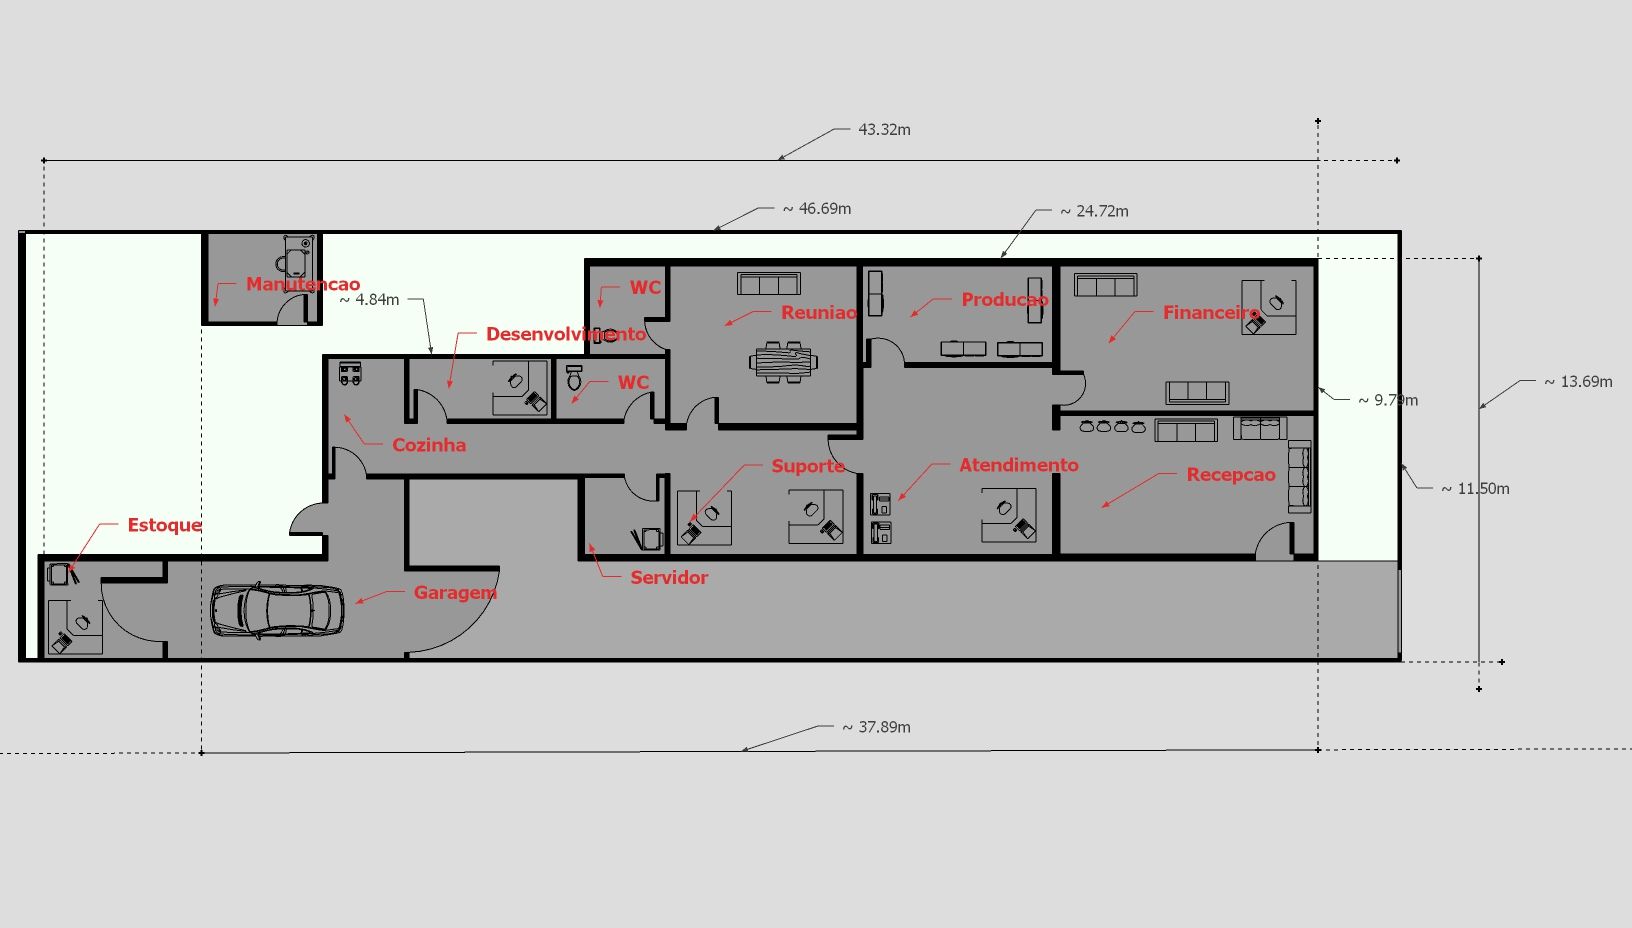
\includegraphics[width=\textwidth]{planta-atual}
	\caption{Planta Atual}
	\label{planta-atual}
\end{figure}

\section{Planta Lógica - Elementos estruturados}

\subsection{Estado atual}
Pegando como base a planta física (Figura \ref{planta-atual}), esboçamos sobre ela a estrutura lógica (Figura \ref{planta-logica-atual}), dos componentes da rede e o caminho percorrido pelos cabos.

\begin{figure}[H]
	\centering
	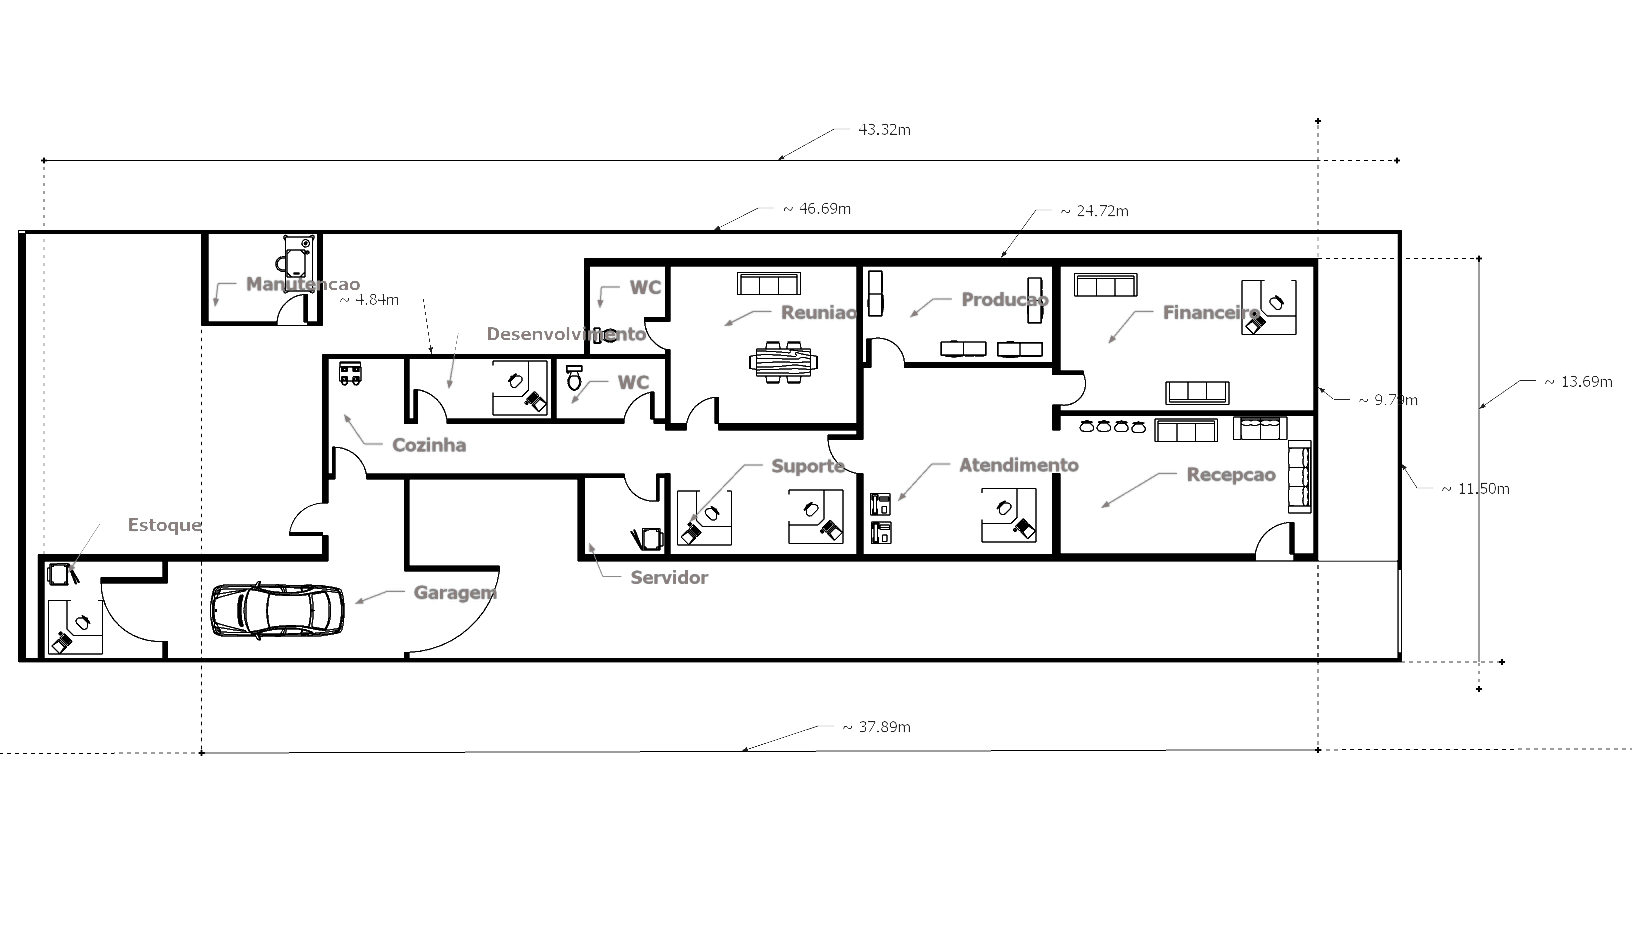
\includegraphics[width=\textwidth]{planta-logica-atual}
	\caption{Planta Lógica Atual}
	\label{planta-logica-atual}
\end{figure}

\subsection{Topologia}

Segundo \cite{senai2012} "O cabeamento estruturado adotou como padrão a topologia estrela, em que
cada tomada de telecomunicação localizada junto ao usuário, deverá estar ligada
a um ponto central que fará a comunicação com a rede de computadores interna
da empresa e à Internet".

Na topologia da Figura \ref{topologia} cada retângulo representa uma sala (Work Area) da planta original. 
Tratando-se de uma topologia estrela, todas as terminações da rede estão advindo da "sala de controle", centralizada na imagem (Figura \ref{topologia}). Que conta com dois Switches (Switch e Switch(1)). Nas salas de "Financeiro", "Reunião" e "Desenvolvimento" há sub-redes de topologia estrela através de um roteador (exemplo: WR$\_$Atendimento).


\begin{figure}[H]
	\centering
	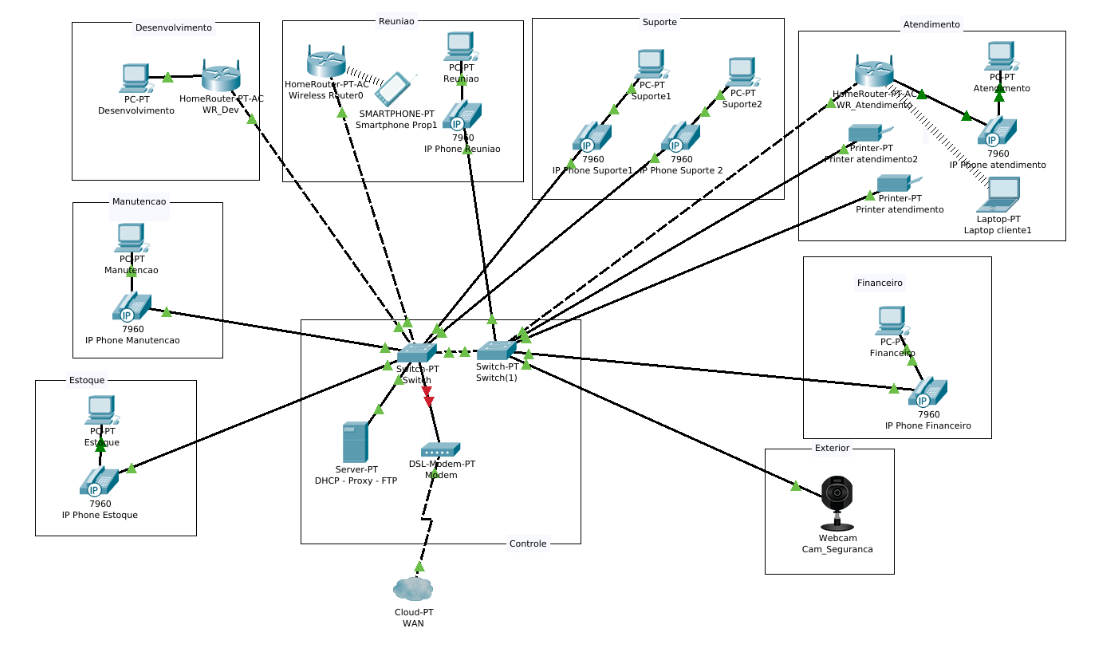
\includegraphics[width=\textwidth]{nova-topologia}
	\caption{Topologia}
	\label{topologia}
\end{figure}

As conexões entre o switch e os end-points representam o cabeamento horizontal, eles estão conectados por cabo de pares trançados de categoria 5e. Observando que a topologia deve estar em conformidade com o padrão de cabeamento estruturado: 
O comprimento máximo entre o segmento de cabo e entre um distribuidor de piso e a tomada de telecomuincações em uma área de trabalho é de 90 metros. As normas de cabeamento estruturado, como a NBR 14565, a ISO/IEC 11801, a ANSI/TIA-568-C.1, entre outras, permitem que os sejam utilizados no subsistema de cabemento horizontal: Cabo de pares trançados Categoria 5e ou superior de quatro pares, 100 oms, U/UTP ou F/UTP; Cabo de fibras ópticas multimode de 50/125 $\mu$m (OM3 e OM4), com duas ou quatro fibras; Cabo de fibras ópticas multimode de 62,5/125 $\mu$m (OM1 e OM2), com duas ou quatro fibras \cite{marin2014cabeamento}.

Algumas terminações foram conectadas através de um IP Phone, como no "IP Phone Financeiro". Esses equipamentos disponibilizam duas portas Ethernet, uma para o switch e outra para um terminal (exemplo: PC), fazendo com que não seja necessário um cabeamento individual para esses dois equipamentos desde o switch. O modem, da sala de controle, deve receber o sinal do provedor de Internet, a conexão WAN poderá ser feita através de cabo de fibra óptica, não especificada na topologia.

Entre os elementos fixos na rede está também a câmera de segurança (Cam$\_$Seguranca), ela está conectada diretamente no switch principal e deverá ter o IP fixado. Os elementos móveis na rede, "Laptop Cliente1" e "Smartphone Prop1" deverão se conectar através das subredes das respectivas áreas de trabalho, mas podendo também transitar entre outras áreas como "Desenvolvimento" e "Atendimento".

A seguir será mostrado o esboço da rack (Figura \ref{diagrama-do-rack}) presente na sala de telecomunicações. O diagrama mostra os equipamentos necessários para o estabelecimento de comércio operar. Tendo como necessidades: VOIP, servidor de arquivos, servidor Proxy, Nobreak etc.

\begin{figure}[H]
	\centering
	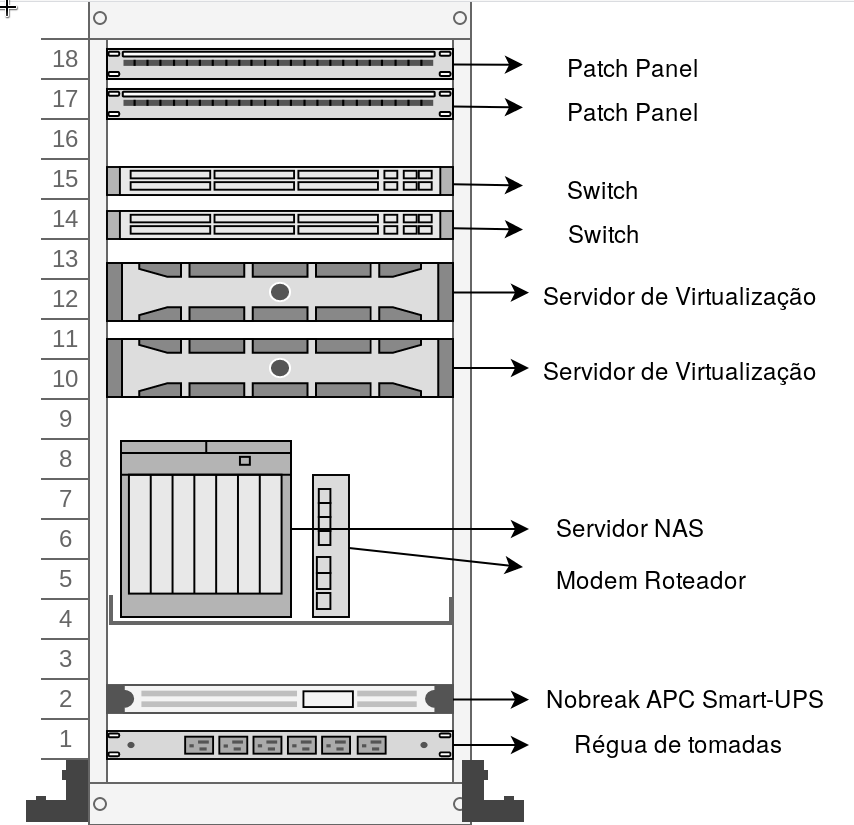
\includegraphics[width=\textwidth]{rack}
	\caption{Diagrama do Rack}
	\label{diagrama-do-rack}
\end{figure}

No projeto foram incluídos dois Patch Panels de 24 portas. Abaixo de cada Patch Panel existe um duto horizontal para organizar os cabos do Patch Panel para o Switch. O segundo patch panel poderá ser usado exclusivamente para conectar telefones IP, considerando-se como sendo uma boa prática. E então conectá-los ao segundo switch para telefonia de serviço PABX. Foram incluídos também, dois servidores para virtualização, esses servidores podem acomodar, dependendo da demanda, serviços como: VOIP, Proxy, DHCP, E-mail, Web etc.

Mais abaixo, está localizado um servidor NAS, utilizado para armazenamento de arquivos de imagens, necessário pois a empresa trabalha com a confecção de crachás e necessita de espaço para armazenamento de imagens processadas e editadas. Na mesma prateleira, ao lado, está o Modem responsável pela conexão WAN vinda da operadora de Internet, que tem a função de roteador, e será conectado ao Switch 1.

Nas duas últimas unidades de espaço da rack estão os ativos de gerenciamento de energia. O Nobreak (UPS) de até 1000 Watts oferece autonomia aos ativos durante quedas de energia de curta e média duração, protege os equipamentos contra sobrecarga, curto-circuito, sobretensões etc. Por último, uma régua de tomadas (PDU) para alimentação de vários equipamentos. A PDU é uma maneira mais simples e prática para solução de alimentação dos ativos na rack, e pode ser conectada diretamente na UPS.

\subsection{Encaminhamento}

Serão utilizadas canaletas de PVC, fixadas nas paredes, descendo do teto, para cobrir os cabos dentro das áreas de trabalho até as tomadas de rede (terminais). Nas áreas de trabalho só serão utilizadas canaletas de PVC, dispensando o uso de aterramento, como é caso das canaletas de metal.

Já para conectar a área de trabalho "Manutenção" que está desmembrada da construção principal (Figura \ref{planta-logica-atual}), será necessário eletroduto de 4 metros de comprimento, com espessura de 3 polegadas. Isso se deve pelo fato desses cabos estarem expostos à condições de estresse pelo clima.

Para o cabeamento horizontal será utilizado o sistema de distribuição de teto. É um sistema constituído por malha de eletrocalhas suspensas no teto, que por meio de postes ou eletrodutos realizam baixadas do teto até os pontos de telecomunicações nas áreas de trabalho \cite{senai2012}.\newpage


\subsection{Memorial descritivo}

\begin{itemize}
	\item Cabos: Para o cabeamento horizontal serão utilizados cabos UTP de categoria 5e, da marca Furukawa. Com extensão máxima de 500 metros e mínima de 300 metros, contando inclusive patch cords;
	\item Conectores: Conectores Fêmea Linkeo RJ45 Cat 5e para tomadas de rede nas áreas de trabalho. Com quantidade mínima de 17 conectores, considerando que cada área de trabalho contará com 2 à 3 tomadas;
	\item Patch Panels: 2 patch panels Linkeo Marca Telecom com 24 conectores RJ45 de categoria 5e;
	\item Rack: Um rack fechado Padrão 19" NetShelter SX 42U, com  profundidade de 1070mm;
	\item Eletrodutos: 3 metros de eletrodutos de PVC para conexão da área de trabalho externa, a área de manutenção; 
	\item Eletrocalhas: Aproximadamente 100 metros de eletrocalha perfurada, tipo "U" de 100x50mm galvanizada. As eletrocalhas formarão a  malha de eletrocalhas suspensas no teto do estabelecimento, com maior ocorrência nos corredores;
\end{itemize}\newpage


\subsection{Identificação dos cabos}

A identificação dos cabos se dará pelo seguinte padrão: \newline

Identificação para Armário/Sala: \newline
 XXA-XX-XX/XX-AAAXXX-XX-XX.\newline

Onde X é carácter numérico e A é carácter alfanumérico.\newline

Exemplo: 

03A-02-21/03-A100-03-01\newline

Origem: andar (03), armário (A), patch panel (02), tomada (21).

Destino: andar (03), sala (A100), espelho (03), posição (01).\newline

Na tabela (Tabela \ref{tabela_identificacao_cabos}) a coluna 'Identificação' mostra o padrão de leitura armário/sala, onde o destino 'ATR' diz respeito a área de trabalho em questão. Por exemplo: ATR001 significa área de trabalho de Suporte.


\begin{table}[H]
\centering
\caption{Tabela de Identificação dos Cabos}
\label{tabela_identificacao_cabos}
\begin{tabular}{|l|l|l|l|}
	\hline
	
	Identificação             & Patch Panel & Sala            \\ \hline
	00A-01-01/00-ATR001-01-01 & 1           & Suporte         \\ \hline
	00A-01-02/00-ATR001-01-02 & 1           & Suporte         \\ \hline
	00A-01-03/00-ATR002-01-01 & 1           & Atendimento     \\ \hline
	00A-01-04/00-ATR002-01-02 & 1           & Atendimento     \\ \hline
	00A-01-05/00-ATR002-02-01 & 1           & Atendimento     \\ \hline
	00A-01-06/00-ATR002-02-02 & 1           & Atendimento     \\ \hline
	00A-01-07/00-ATR003-01-01 & 1           & Recepção        \\ \hline
	00A-01-08/00-ATR004-01-01 & 1           & Financeiro      \\ \hline
	00A-01-09/00-ATR004-01-02 & 1           & Financeiro      \\ \hline
	00A-01-10/00-ATR005-01-01 & 1           & Produção        \\ \hline
	00A-01-11/00-ATR005-01-02 & 1           & Produção        \\ \hline
	00A-01-12/00-ATR006-01-01 & 1           & Reunião         \\ \hline
	00A-01-13/00-ATR006-01-02 & 1           & Reunião         \\ \hline
	00A-01-14/00-ATR007-01-01 & 1           & Desenvolvimento \\ \hline
	00A-01-15/00-ATR007-01-02 & 1           & Desenvolvimento \\ \hline
	00A-01-16/00-ATR008-01-01 & 1           & Manutenção      \\ \hline
	00A-01-17/00-ATR008-01-02 & 1           & Manutenção      \\ \hline
	00A-01-18/00-ATR009-01-01 & 1           & Estoque         \\ \hline
	00A-01-19/00-ATR009-01-02 & 1           & Estoque         \\ \hline
\end{tabular}
\end{table}
\newpage


\section{Implantação}

O cronograma de implantação (Figura \ref{cronograma}) inicia-se no mês de Dezembro, com término previsto para o último dia do mesmo mês. É importante salientar que existem duas etapas de grupos de tarefas no cronograma. A primeira (Cabeamento Estruturado) servirá para instalação do projeto propriamente dito. Por se tratar de uma rede em uso, é importante que a estrutura antiga se mantenha funcionando durante a instalação. Para que na segunda etapa (Remoção Estrutura Antiga), finalmente, se remova a estrutura antiga para descarte e reaproveitamento de ativos da rede.

\begin{figure}[H]
	\centering
	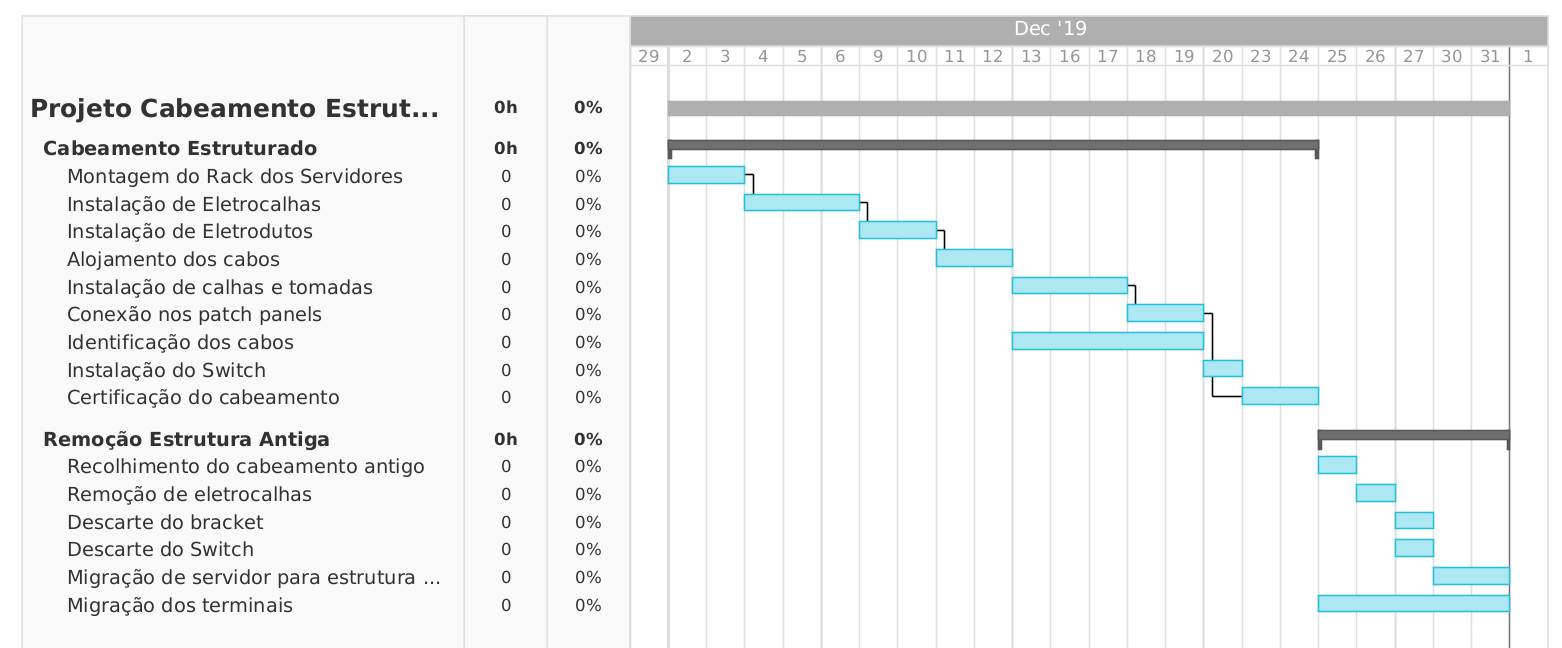
\includegraphics[width=\textwidth]{cronograma}
	\caption{Cronograma de Implantação}
	\label{cronograma}
\end{figure}

As linhas conectando as atividades mostram que a atividade posterior é dependente da anterior, por exemplo, a segunda tarefa de "Instalação de Eletrocalhas" é dependente da primeira atividade de "Montagem do Rack dos Servidores", ou seja, a primeira atividade deve estar concluída para a iniciação da segunda.\newpage

\section{Plano de certificação}

Após a implantação do projeto deve ser feita a certificação do sistema de cabeamento estruturado, a verificação dos passivos, como cabos e conectores, da rede se condizem com as normas de cabeamento estruturado. 

Este processo garante que o trabalho realizado de instalação está seguindo critérios e padrões que asseguram desempenho e qualidade do cabeamento. Para efetuar a certificação é necessário um equipamento especial que executará diversas medidas precisas acerca da funcionalidade e desempenho dos cabos.

Conforme Senai, a certificação de cabeamento estruturado tem como objetivo  aferir os seguintes parâmetros:
\begin{itemize}
	\item Paradiafonia (NEXT, Near End Crosstalk);
	\item Perda de retorno e inserção (atenuação);
	\item Atraso de propagação;
	\item Desvio de atraso de propagação (Delay Skew);
	\item PS-NEXT (Power Sum NEXT);
	\item PS-ELFEXT (Power Sum ELFEXT);
	\item Relação atenuação/paradiafonia (ACR – Attenuation to Crosstalk Ratio);
	\item Entre outros \cite{senai2012};
\end{itemize}

A certificação de rede deve ser feita fora do horário de expediente, entre 18h e 6h da manhã. Desta forma terá a disposição todas as tomadas das áreas de trabalho e patch cords para desconexão, conexão e reparo quando necessário.

A certificação da estrutura deve ser iniciada na sala de telecomunicações. Com o equipamento de certificação devidamente calibrado, deve-se espetar o patch cord no certificador, a seguir, em todas as áreas de trabalho o equipamento remoto deve ser plugado usando um cabo Ethernet de no máximo 5 metros na tomada de rede.

Os parâmetros de testes de par trançado são importantes para verificar fatores que possam obstruir a rede, como o comprimento do cabo, conexão correta, entre outros. Os seguintes testes de cabeamento de par trançado devem ser executados: 

\begin{itemize}
	\item Mapa de fios (Wire Map): Verifica a correta conexão de cada um dos quatro pares, analisando cada um dos oito condutores, se contemplam a configuração 568A ou	568B. O mapa de fios verifica os seguintes itens: continuidade pino a pino, curto-circuito, pares transpostos, pares divididos, condutores abertos e pares invertidos;
	\item Comprimento do cabo: Através da técnica TDR (reflectometria no domínio de tempo) o aparelho envia um pulso elétrico e cronometra o tempo de retorno do pulso entre uma extremidade e outra, a fim de averiguar se a extensão do cabo está condizente com o padrão EIA/TIA 568;
	\item Perda de Inserção (Insertion Loss): diz respeito a atenuação que um sinal sofre durante sua propagação, ela é medida em dB por unidade de comprimento. Essa atenuação se deve pelo fato dos cabos metálicos sofrerem perdas de resistência dos condutores ao longo do filamento;
	\item Diafonia (Crosstalk): refere-se ao nível de interferência eletromagnética entre os pares de condutores de um mesmo cabo, medida em dB. A diafonia não é possível eliminar completamente, mas é possível se chegar a níveis aceitáveis, para isso alguns procedimento podem ser feitos para se chegar a resultados respeitáveis como: perfeita conectorização dos cabos, perfeita conectorização dos patch panels e utilização de cabos e conectores de qualidade. A diafonia se subdivide em paradiafonia (NEXT) e telediafonia (FEXT). O NEXT (Near end Crosstalk) mostra a diafonia ocorrida próxima a conexão do cabo em que a medição está sendo efetuada. Já o PSNEXT (Power sum NEXT) considera a influência de todos os pares de cabo sobre o par que está sendo medido. O FEXT (Far end Crosstalk) é a interferência medida próximo ao
	receptor, ou seja, distante (far) do transmissor. Dentro do FEXT há outra subdivisão em: ELNEXT (atenuação), PSELFEXT (Soma do ELFEXT sobre outros pares de cabo) e PSFEXT (somatória de interferência longe do ponto de medição);
	\item Perda de Retorno: registra a perda de retorno de energia devido às variações de impedância no sistema de cabeamento. Essa perda de retorno é um indicador sobre a qualidade das terminações dos pares de um cabo nas tomadas de telecomunicação;
	\item Atraso de Propagação: está relacionado com o tempo gasto para o sinal percorrer o cabo de uma ponto à outra. Esse atraso tem relação com as características primárias do cabo como: resistência, indutância, capacitância e condutância. Dentro dessa categoria de teste existe também o atraso de propagação relativo (Skew Delay) que é a diferença no tempo que leva o sinal para se propagar pelos condutores no mesmo cabo, isso devido a diferença de comprimento entre os pares de fios torcidos;
	\item Allien Crosstalk: é a interferência de diafonia entre pares de cabos diferentes, isso é possível quando há um agrupamento de muitos cabos, em eletrodutos, eletrocalhas, entre outros. Para minimizar a interferência é recomendado para cada feixe de cabos no máximo 6 cabos;
\end{itemize}

Após os testes executados no certificador, o técnico deve conectar o equipamento num computador e exportar os resultados em PDF e entregar ao cliente. Nos relatórios analíticos são previstos gráficos e tabelas de todos os testes mencionados anteriormente. Nas análises são constados os níveis atuais de cada teste e um paralelo com níveis toleráveis pelas normas de cabeamento estruturado. Bem como, o resultado do teste para cada parâmetro, se foi aprovado ou não.


\section{Plano de manutenção}

Manutenções corretivas, que são aquelas que acontecem depois que o problema ocorreu, se mostram bastante incomodas e caras, pensando nisso, evidencia-se a necessidade de um plano de manutenções preventivas. Apesar da manutenção preventiva aparentar desnecessária e cara num primeiro momento, a longo prazo ela se revela extremamente compensatória e com interessante custo-benefício. Ela evita o comprometimento da infraestrutura e faz o diagnóstico de potenciais erros antes que afetem o fluxo de trabalho organizacional.

O plano de prevenção consiste em manter os equipamentos ativos, passivos e sistemas operacionais funcionando corretamente, executando diagnósticos e análises necessários. Isso inclui: diagnóstico de funcionamento de cabos ponta à ponta, atualização de sistemas operacionais e softwares dos servidores, Backup dos sistemas operacionais, verificação de avarias das tomadas de rede e eletrocalhas de PVC, checagem do estado das baterias do nobreak etc. Ao final de cada período de manutenção deve-se gerar um relatório informativo que conste um histórico de atividades realizadas, assim como os problemas e soluções encontrados. Esses relatórios contribuem para futuros diagnósticos de problemas e para transparência nos processos de auditoria.

Pelo fato da atividade de manutenção de prevenção envolver dedicação e mão de obra especializada, a empresa optará por contratar uma consultoria terceirizada em TI para a operação. Este é o caso de muitas empresas que preferem não alocar os próprios funcionários da empresa para as tarefas de manutenção, afim de não prejudicar a produtividade da empresa. A consultoria, além de providenciar a manutenção periódica da rede, deve contribuir para análises práticas do fluxo de trabalho interno da corporação, sugerindo aperfeiçoamentos que contribuam para as atividades empresariais.

\subsection{Plano de expansão}
Existe um plano de expansão? Quantos novos pontos poderão ser acrecidos na rede, antes de migração de equipamentos na camada 2? Se houver expansão, quais equipamentos deverão ser direcionados para as estremidades da rede? 

\section{Risco}
Enumerar e explicar os riscos do projeto.

\section{Orçamento}
Crie uma relação de orçamentos baseado na seções anteriores.

\section{Recomendações}
Observações e recomendações para o cliente.

\section{Referências bibliográficas}

\renewcommand\refname{} %%Referências bibliográficas}  
\bibliographystyle{apalike}
\bibliography{referencias}  

%% ***********************************************************************
%% === remover daqui =====================================================
%% ***********************************************************************
=================================================
\section{Elementos textuais - Alguns exemplos}

Esta seção apresenta exemplos de elementos textuais. \textbf{Remova-a da versão final do texto}.


\subsection{Colocar elementos em itens}

Texto antes da lista

\begin{itemize}
	\item First item in a list 
	\item Second item in a list 
	\item Third item in a list
\end{itemize}

\subsubsection{Uma subseção de terceiro nivel}

Exemplo de uma subseção

\subsection{Tabelas}

Utilize o site http://www.tablesgenerator.com/ para elaborar as tabelas de seu trabalho.
Para adicionar uma tabela utilize: a tag input, passando o arquivo da tabela como parametro

\begin{table}[h!] % coloque h! para forcar a posicao
\centering
\caption{Modifique a legenda e crie um label}
\label{tab2} %com este label vc faz referencia no texto
\begin{tabular}{|l|l|l|l|l|}
\hline
\multicolumn{1}{|c|}{\textbf{Este é um exemplo de tabela}} & \multicolumn{2}{c|}{\textbf{C1}} & \multicolumn{2}{c|}{\textbf{C2}} \\ \hline
Você pode criar a tabela no excel                          & 1              & 2               & 3               & 4              \\ \hline
Exportar para CSV                                          & 5              & 6               & 7               & 8              \\ \hline
E importar no Table Generator                              & 9              & 10              &                 &                \\ \hline
\multicolumn{5}{|c|}{\textit{Gere o tex, e adicione em seu arquivo}}                                                             \\ \hline
\end{tabular}
\end{table}

Dentro do arquivo você deve definir o label e pode utilizá-lo para referenciar. Exemplo:
Na tab \ref{tab2} temos a relação de ....


Você também pode modificar a tabela manualmente, incluindo, por exemplo h! dentro de sua definição. Veja no exemplo tab2.tex

\subsection{Figuras}



\begin{figure}
\centering
\includegraphics[width=\textwidth]{fig1}
\caption{Exemplo de figura com escala horizontal}
\label{fig1}
\end{figure}


\begin{figure}
	\centering
	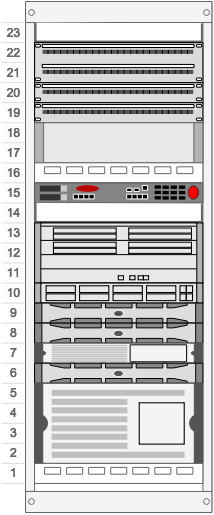
\includegraphics[]{fig2}
	\caption{Exemplo de figura sem escala}
	\label{fig2}
\end{figure}

Você pode rotacionar figuras também. Para isso utilize o parâmetro angle=-90. Repare que a escala da figura foi modificada pelo parametro height. Você também pode utilizar scale

\begin{figure}
	\centering
	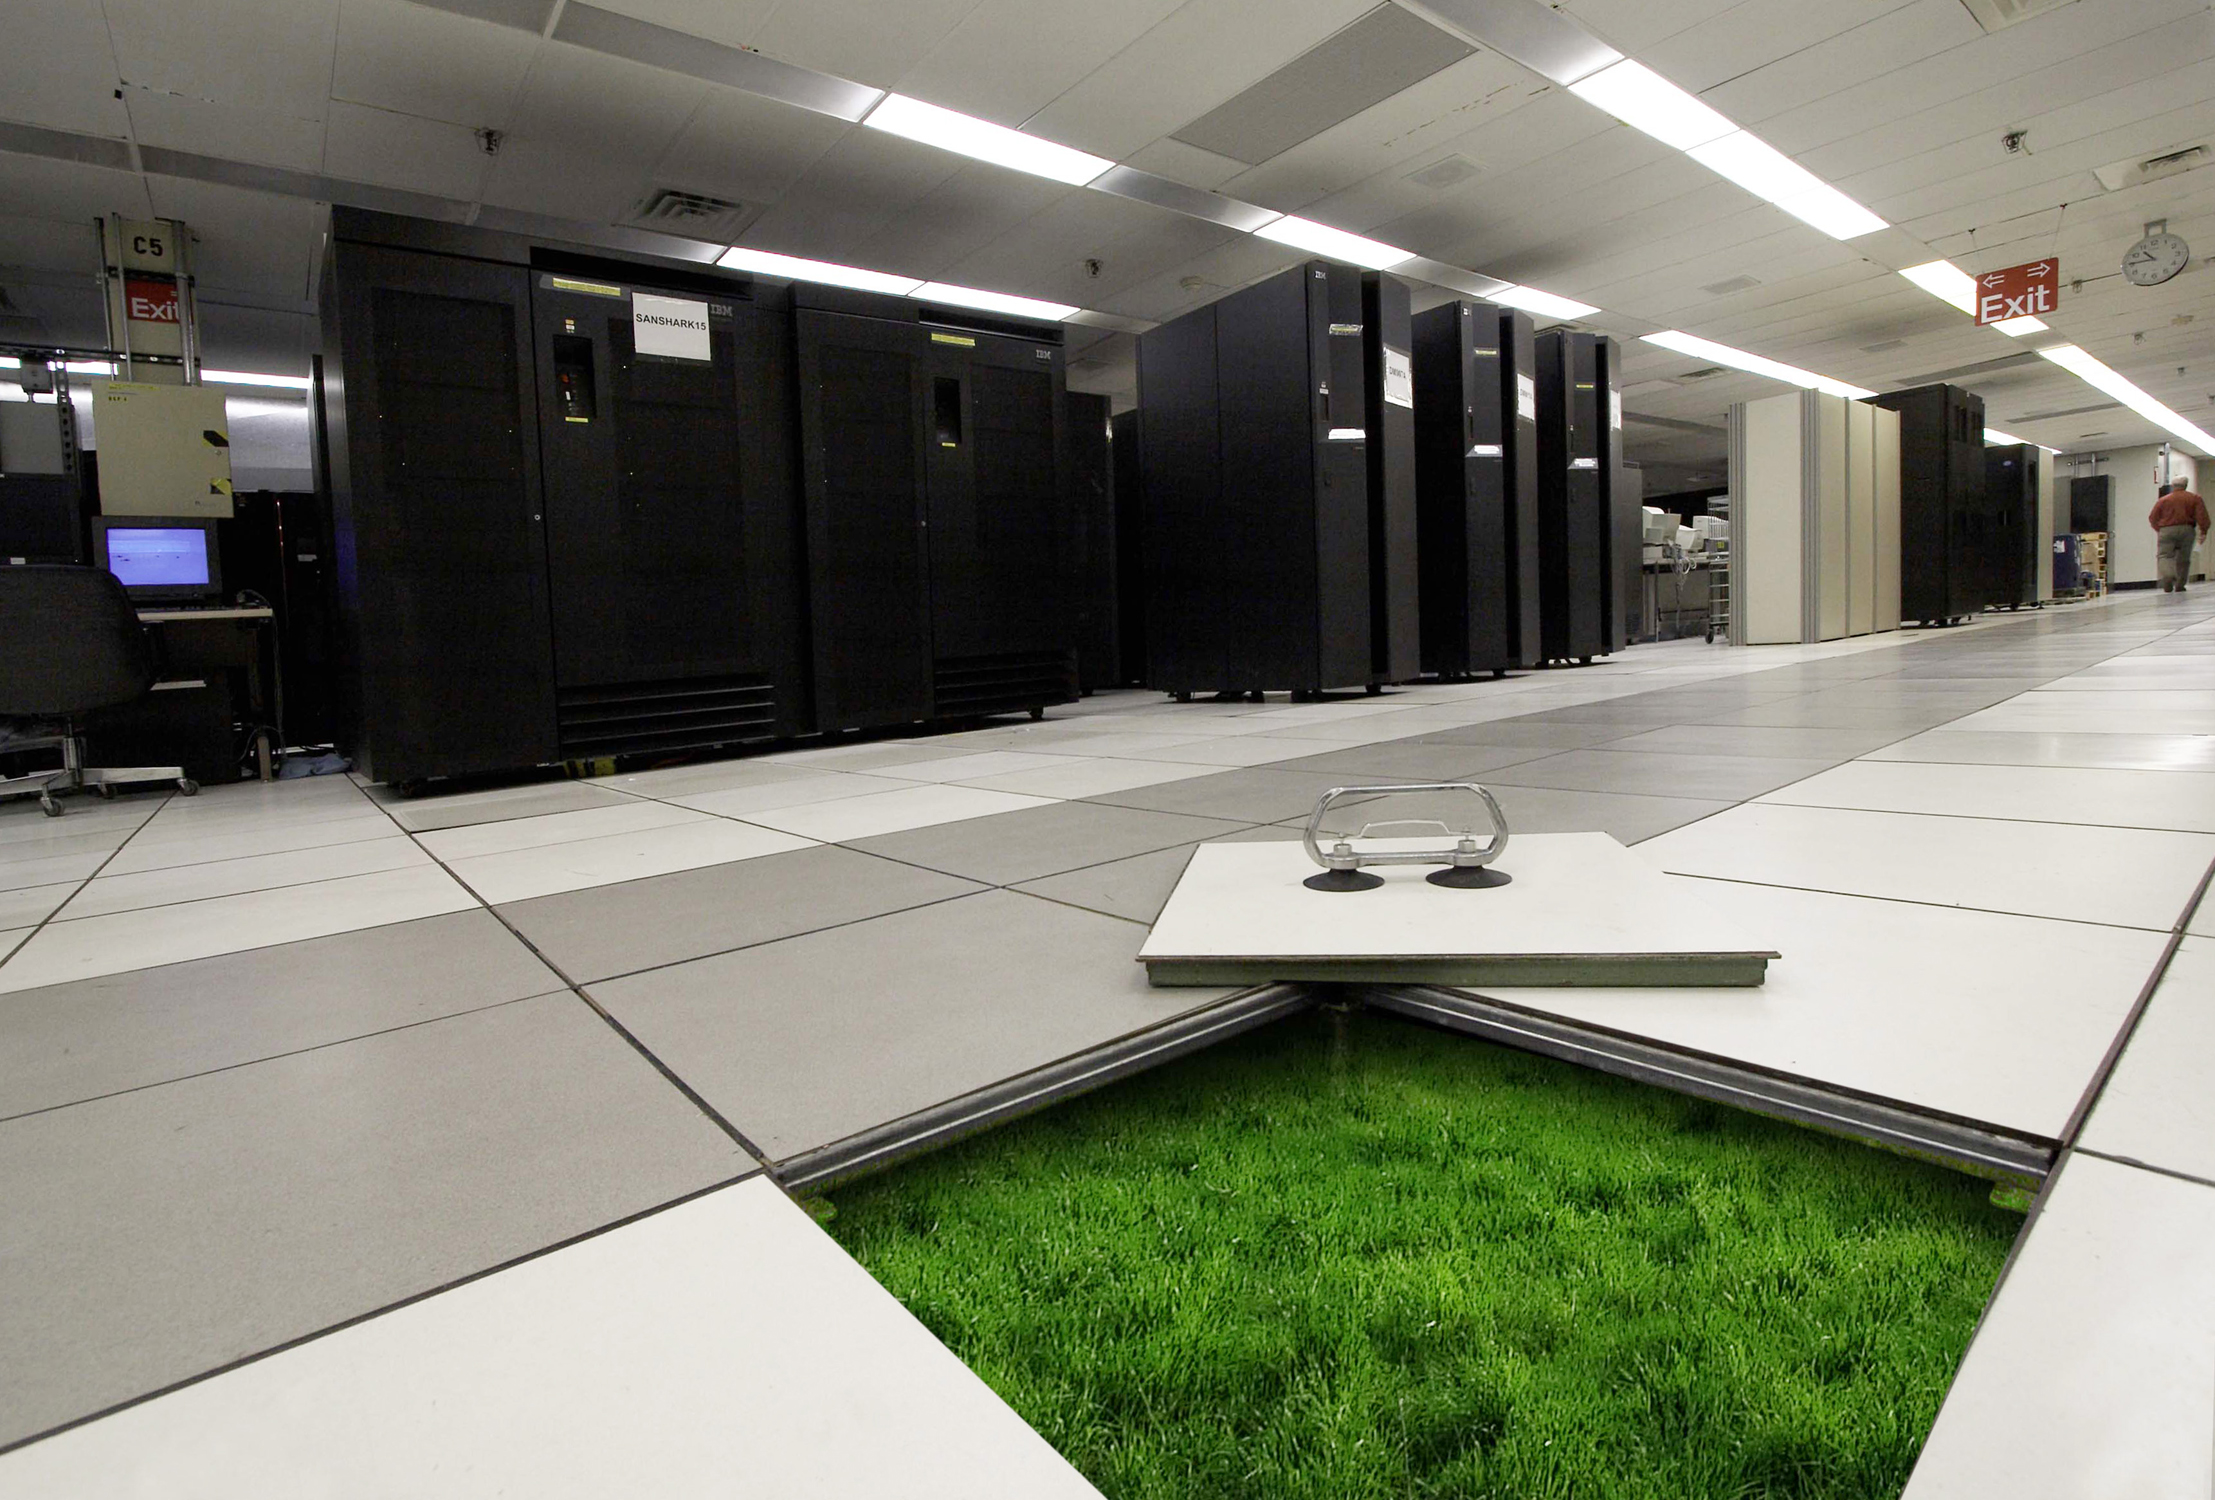
\includegraphics[height=\textwidth,angle=-90]{fig3}
	\caption{Exemplo de figura rotacionada}
	\label{fig3}
\end{figure}

\subsubsection{Resumo gráfico}

Você pode optar por fazer um resumo no formato de mapa mental/conceitual. 
Aqui foi utilizado o site https://app.mindmup.com para gerar o mapa.

Para utilizar o resumo gráfico, remova o texto da seção resumo (linha 137) e inclua o código para inserir a figura, conforme figura \ref{fig4}

\begin{figure}[h]
	\centering
	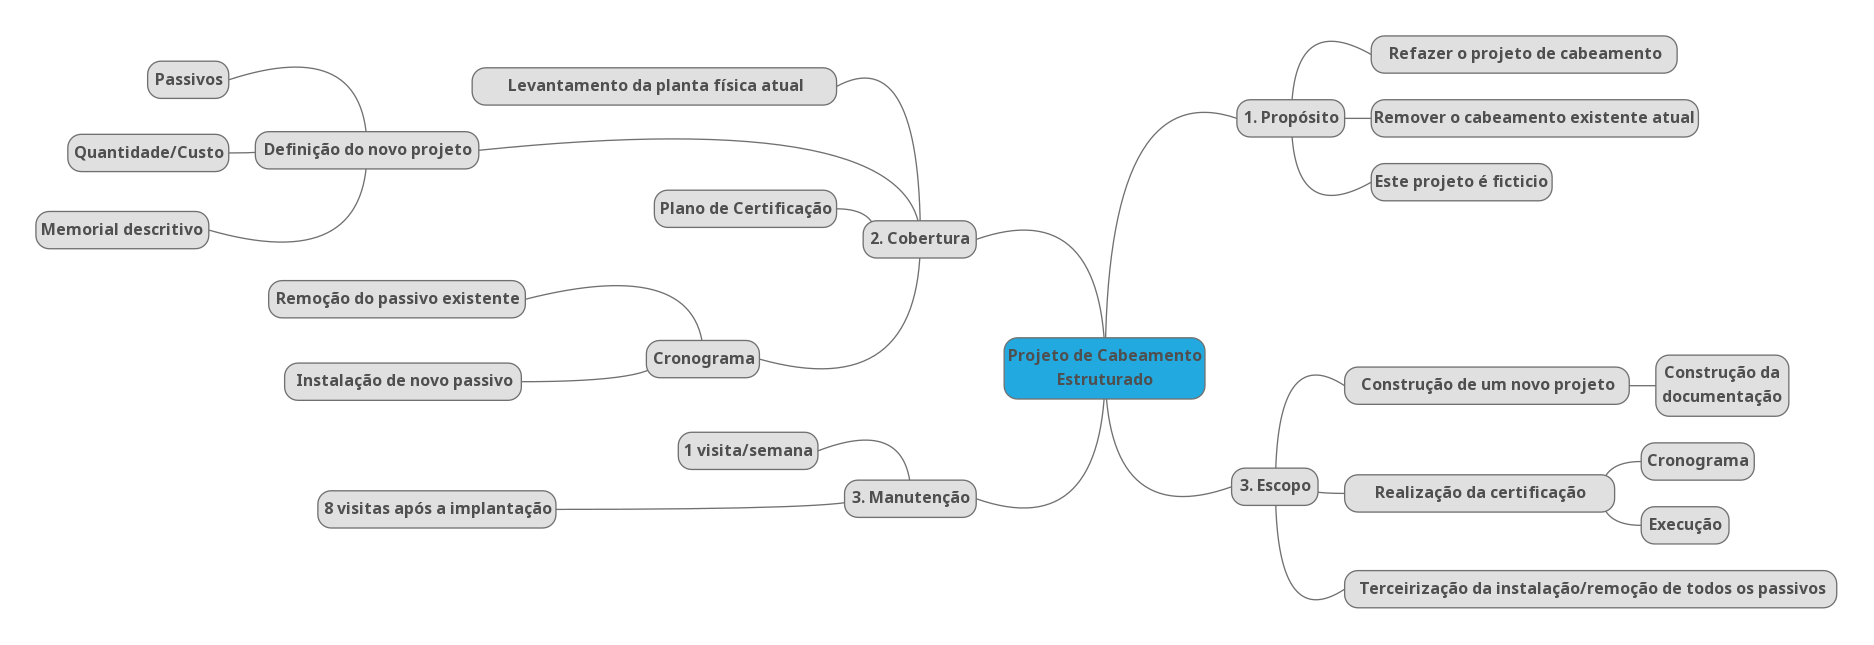
\includegraphics[width=\textwidth,height=5cm,keepaspectratio]{fig4}
	\caption{Exemplo de resumo gráfico}
	\label{fig4}	
\end{figure}

%% ***********************************************************************
%% === ate aqui    =====  ================================================
%% ***********************************************************************

\end{document}